\chapter{Auswirkungen von unterschiedlichen Kameraauflösungen}
\label{sec:minimalAuf} 



Igendwie sagen, dass wie gezeigt wurde der Ansatz für für gleiche Auflösungen funktioniert hat. sRoll im folgendenden die möglichkeit in betracht gezogen werden dass $\zeta \neq \zeta'$. Dazu soll erst einmal erklärt werden, was es für den Sensor bedeutet, wenn sich eine Auflösung ändert und was es bedeutet wenn sich zusätzlich auch noch die Seitenverhältnisse ändern.
%Im vorherigen Kapitel wurde gezeigt, wie eine 3D-Szene aus zwei heterogenen Bildquellen, welche von zwei Kameras gleicher Auflösung aufgenommen wurden, rekonstruiert wurden und gleichzeitig noch die externen Kameraparameter von $C'$ in Relation zu $C$ geschätzt wurden.




Dies wirft die Frage auf, welche Auswirkungen Bilder zweier Kameras mit unterschiedlichen Auflösungen auf die Funktionen den Szenenrekonstruktionsalgorithmus haben. 


Was genau unterschiedliche Auflösungen der Kameras für die einzelnen Bilder bedeutet und was genau sich bei der Aufnahme mit dem Sensor dabei ändert, soll im folgenden Unterkapitel kurz erläutert werden. 

Danach soll analysiert werden, ob eine veränderte Bildauflösung Auswirkungen auf die in Kapitel \ref{sec:HFE} hergeleiteten Abildungsvorschriften hat. Als letztes wird im synthetischen Beispiel die Auflösung einer Kamera mehrmals verändert und der Szenenrekonstruktionsalgorithmus angewandt. Das Ergebnis des Algorithmus wird analysiert und validiert. 

%Danach wird aufgezeigt, was genau diese Veränderungen für die in Kapitel \ref{sec:HFE} Hergeleiteten Bedingungen Epipolargeometrie bedeuten und letztendlich wird das Minimalbeispiel so angepasst, als hätten zwei Kameras unterschiedlicher Auflösung die selbe Szene wie davor aufgenommen und die Resultate miteinander verglichen. 

\section{Abbildungsunterschiede}


Die Geometrie eines Sensors, kann als eine  $M \times N$ - Matrix, bestehend aus $M \times N$  Sensorelementen dargestellt werden\cite{Photonik}. Abbildung \ref{fig:Sensor} zeigt den schematischen Aufbaue eines Sensors (CMOS).

\begin{minipage}{\linewidth}
	\centering
	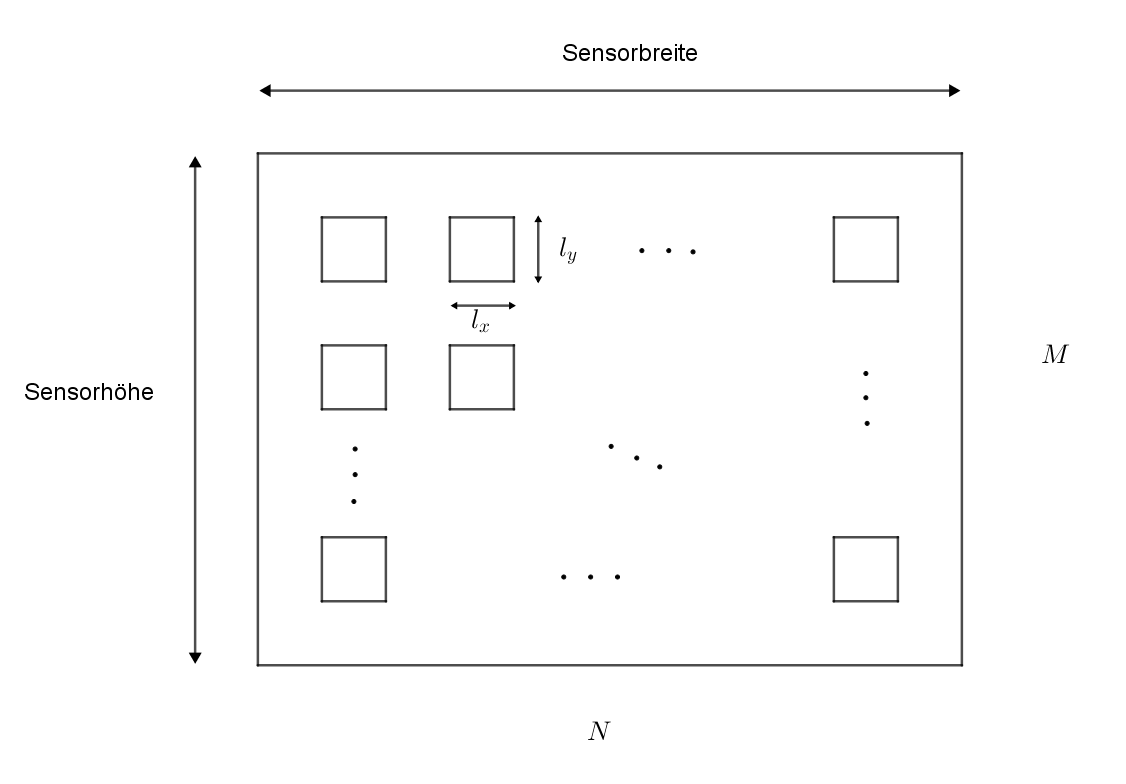
\includegraphics[width=.8\linewidth]{images/Bildsensor_mit_Pixel.png}
	\captionof{figure}{Rechteckiger Bildsensor mit darauf sich befindendenden quadratischen Pixeln. Vlg \cite{Photonik}} 
	\label{fig:Sensor}
\end{minipage}\\ \\


Die Auflösung eines Sensors hängt von den horizontalen und vertikalen Pixelabständen ab und gibt wieder, welche Objektdetails mit dem Sensor gerade noch erkannt werden können.\cite{Photonik}. 


Ein Sensor hat eine maximale Auflösung, welche durch die Anzahl seiner fest installierten Pixel bestimmt wird. Die Bildqualität ist abhängig von der Größe des Sensorchips und der Menge der sich darauf befindenden Pixel. Der CMOS-Sensor einer Canon 6D hat beispielsweise eine Größe von $36 \times 24 mm$ und eine maximale Auflösung von $5.472 \times 3.648$ Pixel. Jedoch ist das nicht die einzige Auflösung, welche beim fotographieren oder filmen mit der Kamera genutzt werden kann. Es können sowohl die Pixelanzahl als auch das Seitenverhältnis der entstehenden Bilder eingestellt werden. Bei der Canon EOS 6D können insgesamt vier verschiedene Seinsverhältnisse eingestellt werden $[3:2], \,[4:3], \,[16:9]$ und $[1:1]$\cite{Canon6D}. Die Bildauflösungen unterscheiden sich pro Seitenverhältnis in sechs Auflösungseinstellungen \textit{L, M, S1, S2, S3}. 

	\begin{table}[h]
	\centering
	\caption{Auflösungen Canon EOS 6D}
	\label{my-label}
	\begin{tabular}{c|c|c|c|c}
		\hline
		\rowcolor{blue!25} 	& 3:2 & 4:3 & 16:9 & 1:1 \\\hline		
		L	&  5478 $\times$ 3648 px & 4864 $\times$ 3648 px & 5472 $\times$ 3072 px & 3648 $\times$ 3648 px \\\hline		
		M &  4104 $\times$ 2736 px & 3648 $\times$ 2736 px & 4104 $\times$ 2310 px & 2736 $\times$ 2736 px \\\hline
		S1 &  2736 $\times$ 1824 px & 2432 $\times$ 1824 px & 2736 $\times$ 1536 px & 1824 $\times$ 1824 px \\\hline
		S2&  1920 $\times$ 1280 px & 1696 $\times$ 1280 px & 1920 $\times$ 1080 px & 1280 $\times$ 1280 px \\\hline
		S3&  720 $\times$ 480 px & 640 $\times$ 480 px & 720 $\times$ 408 px & 480 $\times$ 480 px \\\hline
	\end{tabular}
\caption{Vgl \cite{Canon6D}}
\end{table}

Je geringer die Auflösung, desto geringer ist die Anzahl der Pixel. Die Anzahl der Pixel auf einem Sensorchip kann natürlich nicht variieren. Eine geringere Pixelanzahl bei gleichbleibender Bildgröße, bedeutet, dass sich ein Pixel mit den um sich befindedenden Pixeln interpoliert, so dass ein neuer Pixel bestehend aus mehreren kleinen Pixeln entsteht. Dieser Prozess wird Nachbarschaftsoperation genannt. Für die Berechnung des neuen Bildpixels $px'$ an der Stelle $(m,n)$ wird nicht nur das Bildpixel $p$ des Originalbildes an der Stelle (m,n) verwendet, sondern auch einige seiner Nachbarpunkte\cite{Photonik}. Bei der Canon 6D bietet das Seitenverhältnis $[3:2]$ die Möglichkeit die maximale Pixelanzahl des Sensors zu verwenden, vergleiche hierzu Tabelle 5.1. Bei einem Seitenverhältnis von $[4:3]$ ist die Anzahl der maximal möglichen Pixel nur noch 4864 $\times$ 3648. Änders sich das Seitenverhätnis des Bildauschnitts, so wird auch nicht mehr die gesamte Fläche des Sensors benutzt. 

\begin{minipage}{\linewidth}
	\centering
	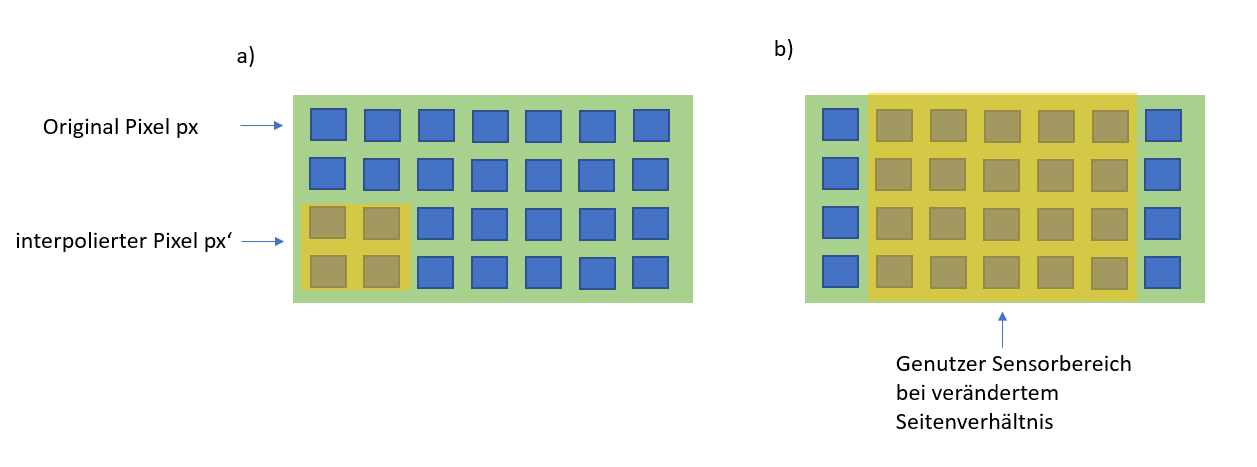
\includegraphics[width=1.\linewidth]{images/AufloesungSensor.png}
	\captionof{figure}{Bild a) zeigt die Interpolation von Pixeln, wenn bei gleichbleibenden Seitenverältnissten weniger Pixel für das Bild verwendet werden sollen. Die interpolierten Pixel leiten dann alle das selbe Signal weiter. Bild b) zeigt in gelb markiert, den verweneten Bereich des Sensors, wenn sich die Seitenverältnisse ändern und nicht mehr der volle Sensor genutzt wird.} 
\end{minipage}\\ \\

\section{Auswirkungen auf die Epipolargeometrie}

Um nun auf die Fragestellung der Auswirkung unterschiedlicher Auflösungen auf die Szenenrekonstruktion zu kommen, kann nun folgende behauptung aufgestellt werden. Beide Kameras besitzen einen Bildsensor, welcher fest in der Kamera installiert ist und sich weder in Position noch seiner Form ändern kann. Dieser Bildsensor beinhaltet sowohl das Bildebenenkoordinatensystem, bei welchem der Hauptpunkt den Koordinatenursprung bildet als auch das Sensorkoordinatensystem, dess Ursprung leicht außerhalb einer der Ecken des Sensors sich befindet. Abbildung ??? zeigt einen Stereoskopischen Szenenaufbau mit Kameras gleicher Auflösung. Die Sensorkoordinatensysteme besitzen die selbe Skalierung. 
\pagebreak
\begin{figure}[!htb]
	\minipage{0.52\textwidth}
	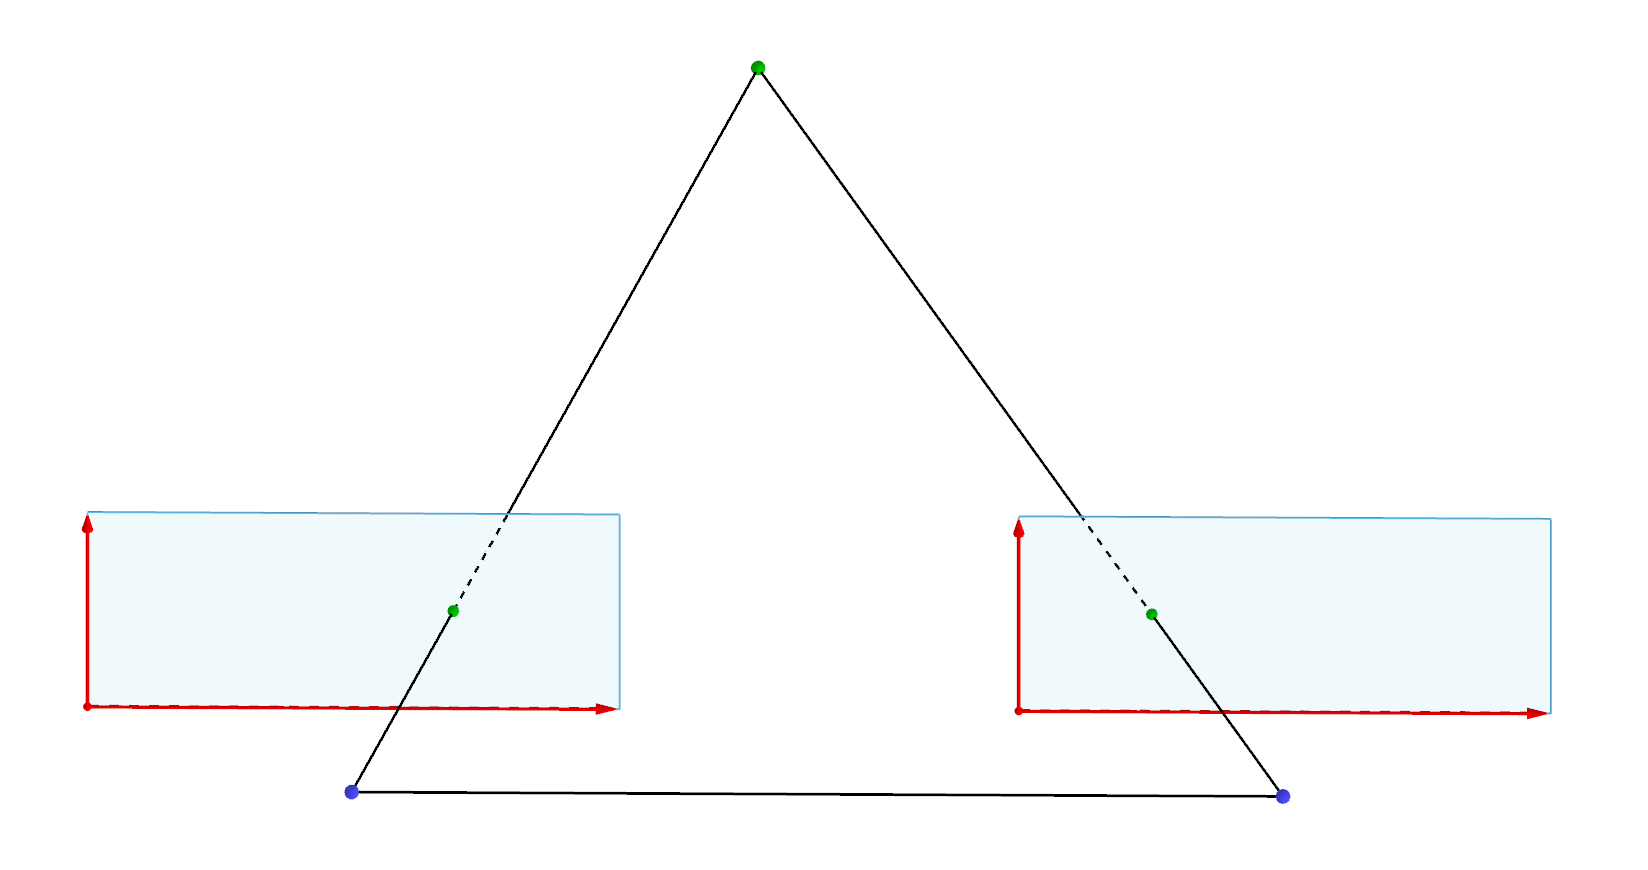
\includegraphics[width=\linewidth]{images/SensorSelbeAufloesung.png}
	\caption{$C$ und $C'$ haben die selbe Auflösung eingestellt}
	\label{fig:awesome_image1}
	\endminipage\hfill
	\minipage{0.52\textwidth}
	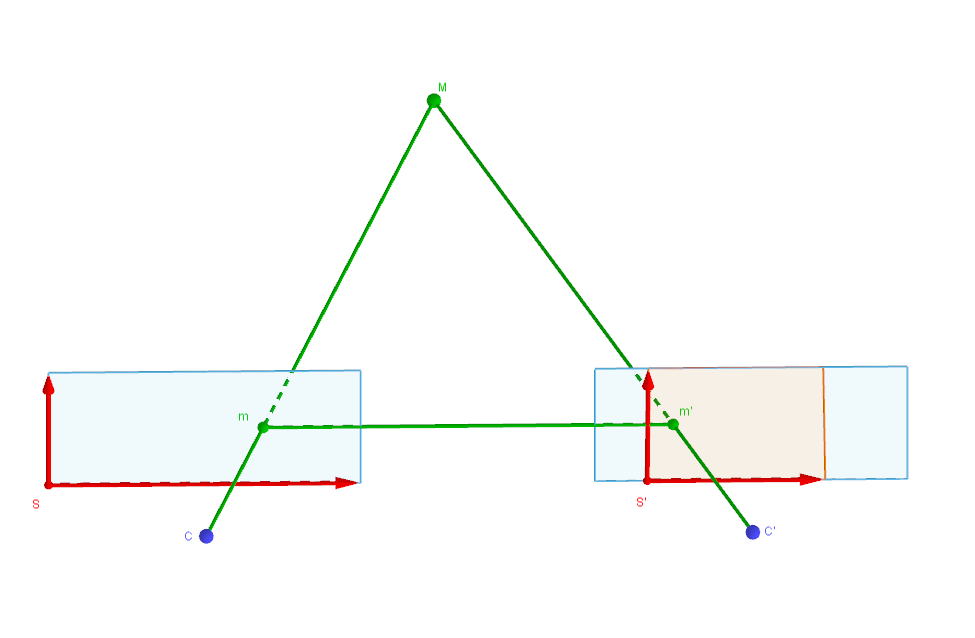
\includegraphics[width=\linewidth]{images/SensorUnterschiedlicheAufloesung.png}
	\caption{$C$ und $C'$ haben unterschiedliche Auflösungen eingestellt}
	\label{fig:awesome_image2}
	\endminipage\hfill
\end{figure}


Es bildet sich wieder das bekannte Dreieck zwischen den Bildpunkten $m_\sigma$ und $m'_{\sigma}$ und dem Objektpunkt $M_\delta$. Das in diesem Falle einen korrekte Szenenrekonstruktion funktioniert, ist im Kapitel \nameref{sec:minimal} anhand des Minimalbeispiels aufgezeigt worden. Wird die Auflösung auf einer der beiden Kameras verringert und damit einhergehend auch noch das Seitenverhältnis geändert, so ändert sich zum einen der aktive Teilbereich des Sensorschips, sowie die Skalierung der Werte auf den Koordinatenachsen des Sensorkoordinatensystems. Die Skalierung der Koordinatenachsen hängt mit der interpolation der mehrerer Pixel zu einem neuen Pixel zusammen. Abbildung 5.3 zeigt schematisch, was sich nach veränderten Auflösungseinstellungen am Sensor verändert.%(GRAFIK EINFÜGEN(hab vergessen welche!))\\
Epipolargeometrisch ändert sich wie man in Abbildung ??? sehen kann nichts. Das zuvor erwähnte Dreieck zwischen den Bildpunkten und dem Objektpunkt bleibt unverändert. Wie in Kapitel \nameref{sec:epipolar} bereits erwähnt, dürfen die Bildebenkoordinatensysteme und somit auch die Sensorkoordinatensysteme unterschiedlich voneinander sein\cite{Elements}. Für die relative Position des Bildpunktes auf dem Sensor ändert sich nichts, dieser bleibt statisch, einzig seine Koordinatenwerte ändern sich im bezug auf das Sensorkoordinatensystems. Für die Fundamentalmatrix und die Essentielle Matrix ergeben sich lediglich andere Vielfache voneinander, welches wie erwähnt ebenfalls gültige Lösungen sind \cite{HZ,Ferid}.

\section{Minimalbeispiel mit unterschiedlichen Kameraauflösungen}

Als Beweise der aufgestellten Behauptung wurde im Minimalbeispiel die Kameramatrix einer der Beiden Kameras unterschiedlich modifiziert. Während für die Kameramatrix von $C$ der Wert $\zeta = -1$ in der Kamermatrix $K$ bleib, wurde das $\zeta$ in $C'$ verändert, so dass sie drei verschiedene neue Kameramatrizen $K'_1, K'_2$ und $K'_3$ ergeben. Die resultierenden Abbildungen des Quaders sind in den Abbildungen ??? bis ??? zu sehen.



\begin{gather}
K = \begin{bmatrix}
-1&0&0&0\\
0&-1&0&0\\
0&0&-1&0\\
%0&0&1&0
\end{bmatrix}\\
K'_1 = \begin{bmatrix}
-2&0&0&0\\
0&-2&0&0\\
0&0&-1&0\\
%0&0&1&0
\end{bmatrix}\\
\end{gather}

\begin{gather}
K'_2 = \begin{bmatrix}
-3.2&0&0&0\\
0&-1.2&0&0\\
0&0&-1&0\\
%0&0&1&0
\end{bmatrix}\\
K'_3 = \begin{bmatrix}
-0.5&0&0&0\\
0&-4.3&0&0\\
0&0&-1&0\\
%0&0&1&0
\end{bmatrix}
\end{gather}\\


\begin{figure}[!htb]
	\minipage{0.48\textwidth}
	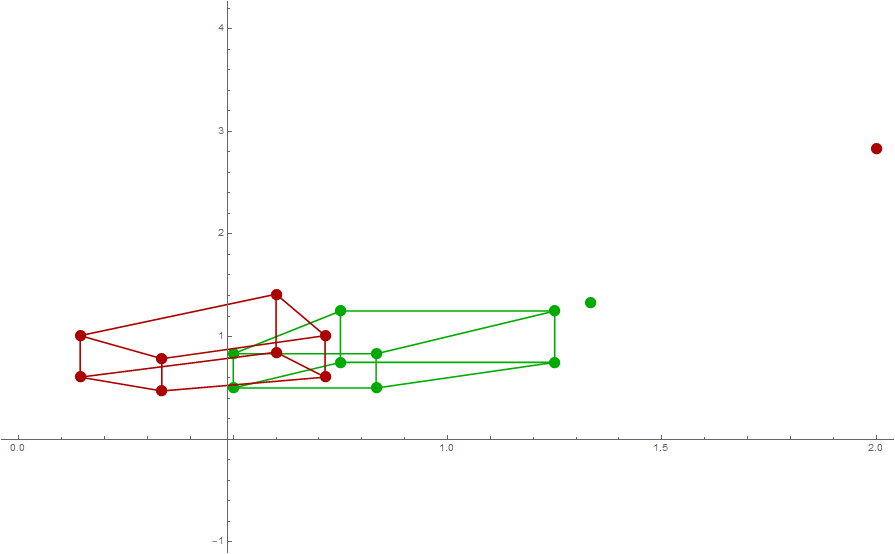
\includegraphics[width=\linewidth]{images/Zeta1.png}
	\caption{$C$ und $C'$ haben die selbe Auflösung eingestellt}
	\label{fig:awesome_image1}
	\endminipage\hfill
	\minipage{0.48\textwidth}
	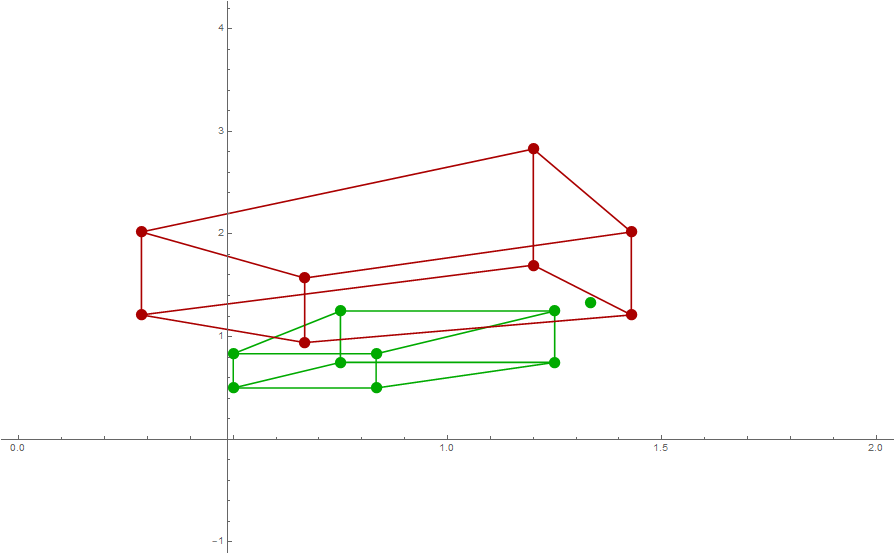
\includegraphics[width=\linewidth]{images/Zeta2.png}
	\caption{$C$ und $C'$ haben unterschiedliche Auflösungen eingestellt}
	\label{fig:awesome_image2}
	\endminipage\hfill
\end{figure}

\begin{figure}[!htb]
	\minipage{0.48\textwidth}
	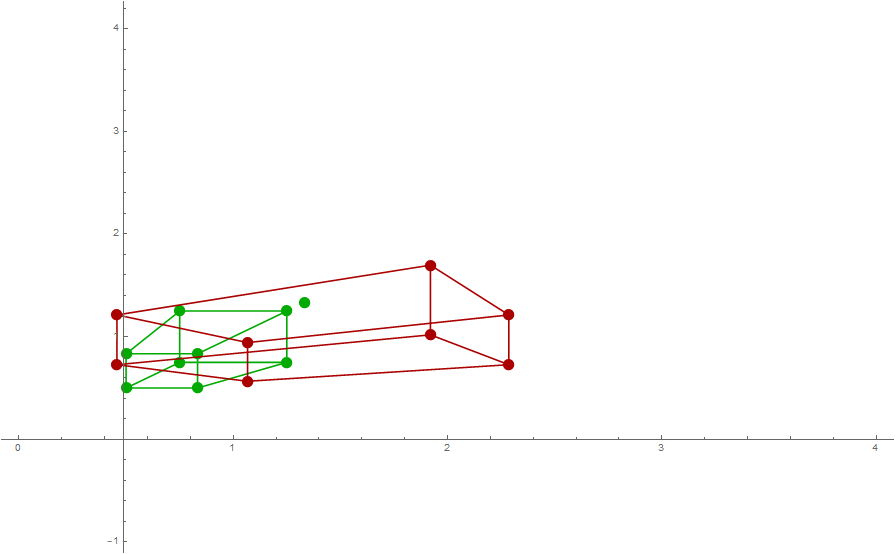
\includegraphics[width=\linewidth]{images/Zeta32_12.png}
	\caption{$C$ und $C'$ haben die selbe Auflösung eingestellt}
	\label{fig:awesome_image1}
	\endminipage\hfill
	\minipage{0.48\textwidth}
	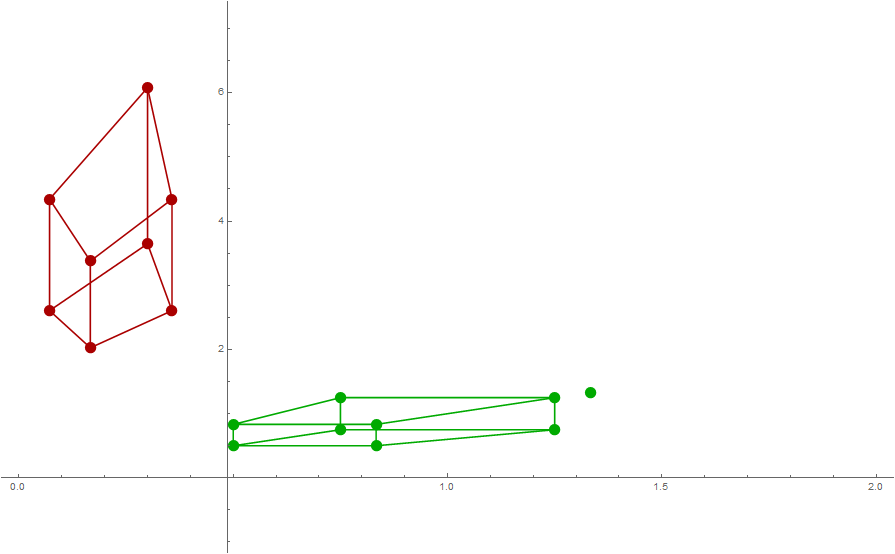
\includegraphics[width=\linewidth]{images/Zeta05_43.png}
	\caption{$C$ und $C'$ haben unterschiedliche Auflösungen eingestellt}
	\label{fig:awesome_image2}
	\endminipage\hfill
\end{figure}


%(GRAFIK $\zeta * 2, \zeta *3,2 und 1.2$, $\zeta * 0.5 und 4.3$ sagen dass das rote jeweils das mit dem verändertem $\zeta$ )\\


Während die Abbildung von $C$ Unverändert bleibt, wird in Abbildung??? Die Abbildung des Quaders in $C'$ ''vergrößert'', was für eine höhere Anzahl an verwendeten Pixeln steht. In Abbildung ??? werden die Pixel in horizontaler Richtung um das 3.2- fache und in vertikaler Richtung um das 1.2-fache erweitert und in Abbilung ??? wird in horzontaler Richtung die Anzahl der Pixel um das 0.5-fache und in vertikaler Richtung um das 4.3-fache skaliert. Für die Fundamentalmatrix und die essentielle Matrix ergeben sich verglichen mit denen aus dem Beipiel mit gleicher Abbildung folgende Matrizen.\\


\begin{gather*}
	\zeta_x = 1, \, \zeta_y = 1: \; \; \;\;
	F = \begin{pmatrix}
			0&-0.5&0\\
			0&0&\frac{1}{\sqrt{2}}\\
			0&-0.5&0
		\end{pmatrix} |: -0.5 \; \leadsto
	F=\begin{pmatrix}
		0&1&0\\
		0&0&-\sqrt{2}\\
		0&1&0
	\end{pmatrix}\\	
	\zeta_x = 2, \, \zeta_y = 2: \; \; \;
	F = \begin{pmatrix}
		0&0.378&0\\
		0&0&-0.534\\
		0&0.756&0
	\end{pmatrix} |: 0.756 \; \leadsto
	F=\begin{pmatrix}
		0&0.5&0\\
		0&0&-\frac{1}{\sqrt{2}}\\
		0&1&0
	\end{pmatrix}\\ \frac{1}{\zeta_x} = 0.5, \;\; \frac{\sqrt{2}}{\zeta_y} = \frac{1}{\sqrt{2}}\\
	\zeta_x = 3.2, \, \zeta_y = 1.2: \; \; \;
F = \begin{pmatrix}
	0&0.198&0\\
	0&0&-0.747\\
	0&0.634&0
\end{pmatrix} |: 0.634 \; \leadsto
F=\begin{pmatrix}
	0&0.312&0\\
	0&0&-1.178\\
	0&1&0
\end{pmatrix}\\ \frac{1}{\zeta_x} = 0.312, \;\; \frac{\sqrt{2}}{\zeta_y} = -1.178\\
	\zeta_x = 0.5, \, \zeta_y = 4.3: \; \; \;
F = \begin{pmatrix}
	0&0.885&0\\
	0&0&-0.145\\
	0&0.442&0
\end{pmatrix} |: 0.442 \; \leadsto
F=\begin{pmatrix}
	0&2&0\\
	0&0&-0.328\\
	0&1&0
\end{pmatrix}\\ \frac{1}{\zeta_x} =2, \;\; \frac{\sqrt{2}}{\zeta_y} = -0.328
\end{gather*}\\

%\begin{minipage}{\linewidth}
%	\centering
%	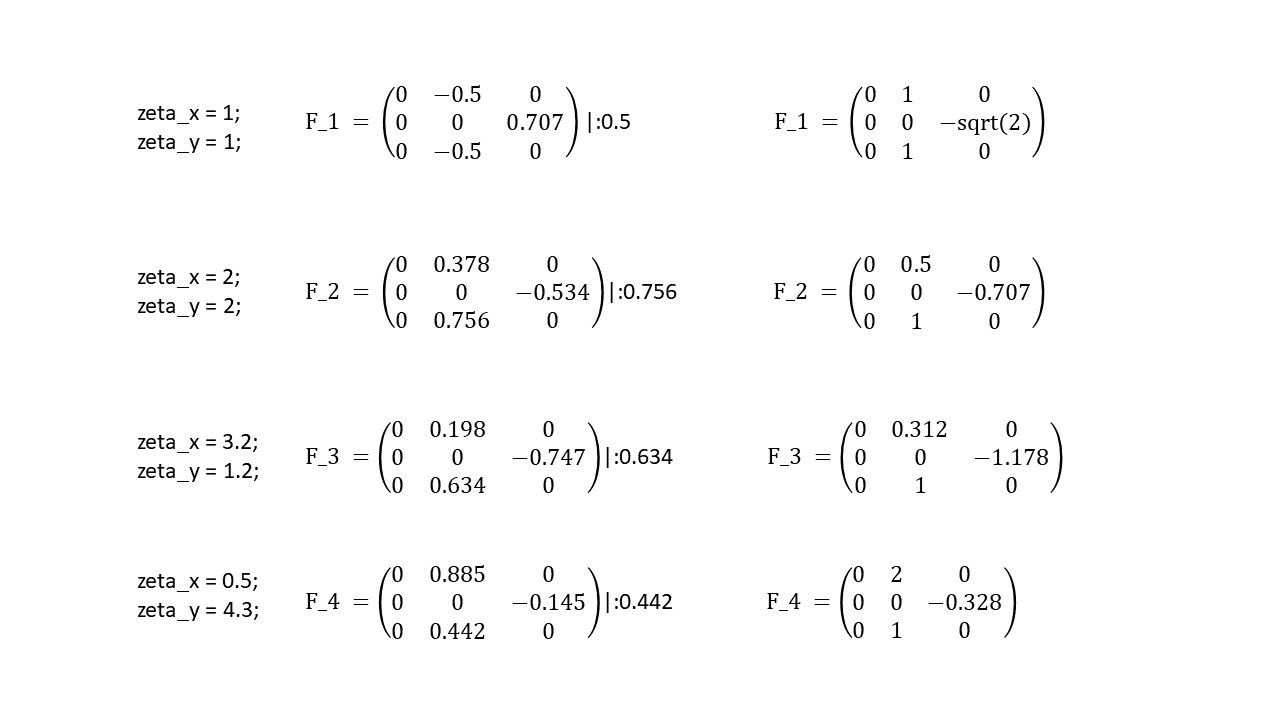
\includegraphics[width=1.\linewidth]{images/FundEMatrizen.png}
%	\captionof{figure}{Die Fundamentalmatrizen sind bei jeder Auflösung, die gewählt wurden immer Vielfache voneinander} 
%\end{minipage}\\ \\
(hier können vllt noch die verschiedenen rotationen gezeigt werden ,welche immer die selbe rotation bewirken)
Die Werte für $\zeta_x$ wirken sich auf die erste Zeile der Fundamentalmatrix aus, während die Werte von $\zeta_y$ sich auf die zweite Zeile auswirken. Bei der nachfolgenden Umrechnung der Fundamentalmatrix in die essentielle Matrix mit Hilfe der Kameramatrizen $K$ und $K'$, kann gestgestellt werden, dass die Ergebnisse jeweils Vielfache voneinander sind. \\


\begin{gather*}
		\zeta_x = 1, \, \zeta_y = 1: \; \; \;\;
	E = \begin{pmatrix}
		0&-0.5&0\\
		0&0&\frac{1}{\sqrt{2}}\\
		0&0.5&0
	\end{pmatrix} |: 0.5 \; \leadsto
E = \begin{pmatrix}
	0&-1&0\\
	0&0&-\sqrt{2}\\
	0&1&0
\end{pmatrix}\\
		\zeta_x = 2, \, \zeta_y = 2: \; \; \;\;
E = \begin{pmatrix}
	0&0.756&0\\
	0&0&1.069\\
	0&-0.756&0
\end{pmatrix} |: -0.756 \; \leadsto
E = \begin{pmatrix}
	0&-1&0\\
	0&0&-\sqrt{2}\\
	0&1&0
\end{pmatrix}\\
		\zeta_x = 3.2, \, \zeta_y = 1.2: \; \; \;\;
E = \begin{pmatrix}
	0&0.634&0\\
	0&0&1.069\\
	0&-0.634&0
\end{pmatrix} |: -0.634 \; \leadsto
E = \begin{pmatrix}
	0&-1&0\\
	0&0&-\sqrt{2}\\
	0&1&0
\end{pmatrix}\\
		\zeta_x = 0.5, \, \zeta_y = 4.3: \; \; \;\;
E = \begin{pmatrix}
	0&0.442&0\\
	0&0&1.069\\
	0&-0.442&0
\end{pmatrix} |: -0.442 \; \leadsto
E = \begin{pmatrix}
	0&-1&0\\
	0&0&-\sqrt{2}\\
	0&1&0
\end{pmatrix}\\
\end{gather*}

%\begin{minipage}{\linewidth}
%	\centering
%	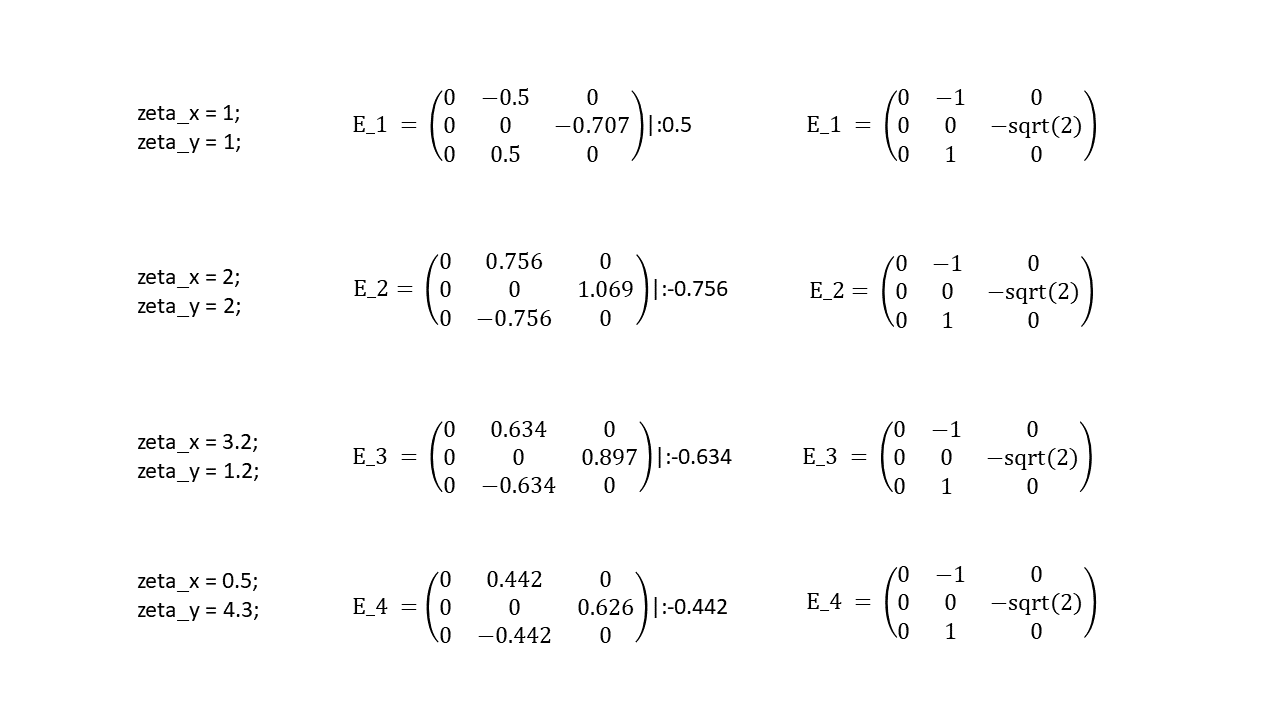
\includegraphics[width=1.\linewidth]{images/EMatrizen.png}
%	\captionof{figure}{Die essentiellen Matrizen sind bei jeder Auflösung, die gewählt wurden immer Vielfache voneinander} 
%\end{minipage}\\ \\

Bei der Rekonstruktion der externen Kamerparameter ergibt sich daraus stehts die selbe Matrix für $P'$. Was wie gezeigt daran liegt, dass sich geometrisch nichts ändert, sondern lediglich die skalierung der Koordinatenwerte der Bildpunkte und somit auch eine Skalierung der Einträge in $F$ und $E$, welche aber ebenfalls als Skaleninvariant definiert sind\cite{HZ}. Die Ergebnisse der darauffolgenden Szenenrekonstruktionen, der einzelnen Szenen zeigt, dass sich immer die selbe Szene ergibt, welche mit der eigens aufgebauten Szene übereinstimmen.\\


\begin{minipage}{\linewidth}
	\centering
	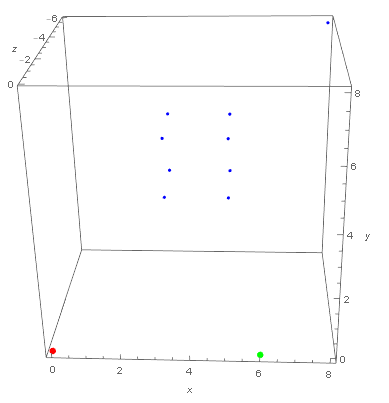
\includegraphics[width=0.5\linewidth]{images/DifferentAufloesungRekonstructedScene.png}
	\captionof{figure}{Die rekonstruierten Szenenpunkte und Kamerapositionen bleibt auch bei unterschiedlichen Auflösungen die selben} 
\end{minipage}\\ \\

Die Behauptung, dass die Auflösung der Kamera bei dem in dieser Arbeit gewählten Workflow für die Rekonstruktion der Szene keine Auswirkung hat, kann für das Minimalbeispiel bestätigt werden. \\




%(NICHT LÖSCHEN!DAS GEHÖRT ALLES IN KAPITEL 7!!!)
%Wenn man sich mit digitalen Bilddaten auseinandersetzt, so kommt man nicht drum herum sich auch mit den verschiedenen Auflösungsarten beschäftigen zu müssen.
%Aus der Stereokalibrierungsapp, welche \textit{MatLab} anbietet, ist bekannt, dass diese nicht mit Bildern unterschiedlicher Auflösung eine Szenerekonstruktion durchführen kann. 
%Der erste Schritt bestand erstmal darin zu überprüfen, warum zwei unterschiedliche Auflösungen in \textit{MatLab} Probleme machen. \textit{MatLab} verfolgt einen etwas anderen Rekonstruktionsansatz. Zu aller erst werden die Kameras kalibriert. Dies geschieht über die Matlab-Funktion \text{estimateCameraParameters}\cite{MatlabCamParam}. 
%Diese Funktion funktioniert auch bei Bildern unterschiedlicher Auflösung noch ohne Probleme. Das Problem, welches sich als eigentlich minimales Problem herausstellt, ist, dass die darauf folgenden Rektifizierung der Stereobilder nicht mit zwei Bildern unterschiedlicher Auflösung funktioniert. 
%In den \textit{MatLab} references, steht es nicht expliziet drin \cite{MatlabRec}. Die Rektifizierung in Matlab funktioniert nach einem Schema, welches ähnlich dem aufgezeigten Beispiel im Kapitel \nameref{sec:rectification} bereits erwähnt wurde und in \cite{Fusiello,FusielloSite} nochmal genau aufgeführt wird.
% Das Problem liegt also nicht daran, dass bilder unterschiedlicher Auflösung nicht rektifiziert werden können, sondern das Problem liegt an dem in \textit{MatLab} verwendeten Algorithmus für die Rektifizierung zweier Stereobilder (Foren Zitieren????). Warum \textit{MatLab} überhaupt rektifiziert, liegt daran, dass ein Ansatz der Szenerekonstruktion gewählt wurde, welcher die essentielle Matrix nicht benötigt. In diesem Falle, werden zwei Stereobilder aufgenommen, danach rektifiziert und anschließend über eine sogenannte \textit{Disparity-Map}, die Szenen punkte rekonstruiert\cite{MatlabDisp,MatlabStereoApp,Fusiello,Javier}. 
%Der in dieser Arbeit gewählte Rektifizierungsalgorithmus, ist nicht auf gleiche Kameraauflösungen beschränkt. Mittlerweile gibt es natürlich deutlich fortgeschrittenere Rektifizierungsansätze, jedoch wurde für diese Arbeit der Ansatz von \cite{ZZ} gewählt, um ein Gefühl zu vermitteln, dass wenn man sich auf die Epipolargeometrie bezieht, die Auflösungen der Kameras keine Rolle spielen\cite{Elements}.

